\chapter*{Đặt vấn đề}\label{chap1}
\addcontentsline{toc}{chapter}{Đặt vấn đề}
Kiểm thử và đảm bảo chất lượng phần mềm là một phần quan trọng trong quá trình phát triển phần mềm \cite{GiaoTrinhKiemThu}. Ngày nay, với sự phát triển mạnh mẽ của công nghệ, vai trò của kiểm thử ngày một thiết yếu hơn khi cuộc sống con người gắn liền với các phần mềm, các thiết bị điện tử thông minh bởi chúng hỗ trợ, đáp ứng các nhu cầu thiết yếu trong cuộc sống. Trong đó, các dự án nhúng viết bằng C/C++ đã và đang tạo ra các sản phẩm phần mềm thông minh cần thiết cho người dùng~\cite{plauger1997embedded}. Với sự phát triển của ngành công nghiệp ô tô, các dự án nhúng C/C++ đang dần xuất hiện trong các phần mềm điều khiển trên xe hơi \cite{gassmann2019towards}. Để đảm bảo an toàn cho người dùng khi sử dụng các sản phẩm phần mềm, chất lượng mã nguồn cần được đảm bảo một cách chính xác theo các tiêu chuẩn nghiêm ngặt như ISO (ISO-9126~\cite{ali2017iso}, ISO-26262~\cite{Hillenbrand2012_1000025616}) hay MISRA-C\footnote{https://misra.org.uk/misra-c/}. Thực tế cho thấy rằng phần lớn các dự án nhúng C/C++ có cấu trúc mã nguồn phức tạp, kích thước lớn và có nhiều sự tương tác giữa các mô-đun. Bởi vậy, để phát hiện sớm các lỗi phát sinh, quá trình kiểm thử thường được triển khai từ sớm, ngay cả khi mã nguồn chưa đầy đủ, mới chỉ có các lớp giao diện được đề ra bởi lập trình viên. Phương pháp kiểm thử thủ công bộc lộ nhiều khó khăn, tiêu tốn nhiều thời gian và chi phí khi triển khai kiểm thử từ sớm như vậy bởi quá trình kiểm thử đi kèm việc tạo giả lập mã nguồn cho các đơn vị chưa được cài đặt. Do đó, việc kiểm thử tự động cho các dự án nhúng C/C++, ngay cả khi mã nguồn chưa đầy đủ, đã và đang trở thành thách thức lớn được không chỉ cộng đồng nghiên cứu mà còn được các công ty phát triển phần mềm quan tâm.

Kiểm thử phần mềm tự động đã và đang được áp dụng rộng rãi nhằm giảm thiểu chi phí của quá trình kiểm thử. Các kỹ thuật kiểm thử tự động dựa trên đồ thị dòng điều khiển (Control Flow Graph - CFG) và đồ thị dòng dữ liệu là hai hướng nghiên cứu chính được nhiều nhà nghiên cứu quan tâm. Trong đó, kỹ thuật kiểm thử tự động dựa trên CFG được sử dụng phổ biến với hai hướng tiếp cận chính là kiểm thử tĩnh \cite{SecureProgrammingWithStaticAnalysis, Buckle:1998:StaticAnalysisofSafetyCriticalSoftwareTechniquesToolsandExperiences} và kiểm thử động \cite{Grigorenko:1998:DynamicTesting, TUNG2022106821}. Mỗi hướng tiếp cận đều có ưu, nhược điểm riêng nhưng nhìn chung đều mang lại hiệu quả cao trong việc đảm bảo chất lượng phần mềm. Cụ thể, kiểm thử tĩnh tập trung vào việc sinh dữ liệu kiểm thử dựa trên quá trình phân tích mã nguồn mà không cần chạy chương trình. Kĩ thuật kiểm thử tĩnh cung cấp nhiều lợi ích khi kĩ thuật này có thể áp dụng sớm trong vòng đời phát triển phần mềm, từ đó phát hiện sớm các lỗi phát sinh, các sai sót trong đặc tả, giúp giảm thời gian và công sức kiểm thử. Tuy nhiên, kiểm thử tĩnh có một số nhược điểm như yêu cầu nhiều tài liệu liên quan, không phát hiện được lỗi tiềm ẩn trong quá trình chạy. Do vậy, hướng tiếp cận này khó có thể tiến hành tự động hoàn toàn. Kiểm thử động là hướng tiếp cận kiểm thử dựa trên việc thực thi chương trình để phát hiện lỗi tiềm ẩn, sai sót trong cài đặt so với đặc tả. Hai hướng tiếp cận có những ưu, nhược điểm bổ trợ cho nhau nên chúng thường được áp dụng đồng thời trong quá trình kiểm thử. 

Kế thừa hai hướng tiếp cận trên, Godefroid và cộng sự đã đề xuất phương pháp kiểm thử tượng trưng động \cite{ConcolicTesting}, cài đặt trong công cụ DART~\cite{DART}, nhằm khắc phục nhược điểm và tận dụng những ưu điểm của kiểm thử tĩnh và kiểm thử động. Quá trình sinh dữ liệu kiểm thử trong phương pháp này bao gồm ba pha chính: (i) sinh dữ liệu kiểm thử khởi tạo, (ii) thực thi dữ liệu kiểm thử và phân tích đường thi hành, và (iii) sinh dữ liệu kiểm thử có hướng. Phương pháp bắt đầu bằng việc sinh ngẫu nhiên dữ liệu kiểm thử khởi tạo. Sau khi thực thi dữ liệu kiểm thử ngẫu nhiên, đơn vị kiểm thử có thể tồn tại một số câu lệnh và nhánh chưa được viếng thăm. Để giải quyết vấn đề này, kiểm thử tượng trưng động chọn một đường thi hành chưa được viếng thăm trên CFG của đơn vị kiểm thử. Điều này cho phép phương pháp sinh dữ liệu kiểm thử có hướng, nhằm phủ đường thi hành đó. Phương pháp này có khả năng đạt được độ phủ mã nguồn cao hơn so với các hướng tiếp cận truyền thống. Trong thực tế, kiểm thử tượng trưng động đã và đang được ứng dụng trong nhiều dự án với mục tiêu tăng cường độ phủ mã nguồn và phát hiện lỗi chương trình với chi phí thấp. Kiểm thử tượng trưng động sau đó thu hút sự quan tâm lớn từ cộng đồng nghiên cứu và các công ty phát triển phần mềm. Minh chứng là sự ra đời của một số công cụ kiểm thử dựa trên kĩ thuật tượng trưng động như CUTE~\cite{CUTE}, PathCrawler~\cite{PathCrawler}, CAUT~\cite{CAUT}, SDART~\cite{SDART}, VFP~\cite{TUNG2022106821}, v.v. Hơn nữa, một số phương pháp khác như EXE~\cite{EXE}, KLEE~\cite{KLEE}, hay KLOVER~\cite{li2011klover}, thay vì thực thi chương trình với dữ liệu đầu vào được sinh thủ công hoặc ngẫu nhiên, đã áp dụng kiểm thử tượng trưng động để sinh dữ liệu đầu vào có giá trị tượng trưng có thể gây lỗi chương trình.

Hiện nay, dù đã có nhiều nghiên cứu xoay quanh kiểm thử tượng trưng động cho mã nguồn C/C++ nhưng vẫn tồn tại một số hạn chế khi áp dụng phương pháp trong quá trình kiểm thử đơn vị. Trong đó, một số hạn chế bắt nguồn từ việc mã nguồn kiểm thử chưa đầy đủ. Trong vòng đời phát triển phần mềm, mã nguồn trong pha cài đặt thường bắt đầu với việc đội ngũ lập trình viên thiết kế, đặc tả và cài đặt các lớp giao diện, kiểu dữ liệu trừu tượng, v.v. Mục đích của việc này là để các thành viên trong đội nhóm phát triển biết được dịch vụ sẽ được cung cấp bởi các thành phần trong mã nguồn, qua đó đẩy nhanh tốc độ cài đặt thành phần được giao. Điều này dẫn tới hạn chế đầu tiên đó là mã nguồn có thể chứa hàm thiếu định nghĩa. Hàm thiếu định nghĩa là những hàm mà có nguyên mẫu được khai báo, nhưng không có định nghĩa hàm. Điều này có thể xuất hiện khi nhóm phân chia công việc và mỗi thành viên chịu trách nhiệm về việc triển khai một số hàm cụ thể. Tuy nhiên, việc quản lý và theo dõi những hàm này trong quá trình phát triển và kiểm thử có thể gây khó khăn, đặc biệt khi số lượng hàm thiếu định nghĩa lớn. Bài toán trở nên phức tạp hơn khi áp dụng kiểm thử tự động bởi các công cụ kiểm thử tự động thường đòi hỏi mã nguồn đầy đủ để thực thi các ca kiểm thử. Chương trình chứa các hàm thiếu định nghĩa có thể biên dịch được nhưng không thể liên kết các tệp đối tượng để tạo thành một tệp thực thi. Theo nghiên cứu của khóa luận, hiện nay chưa có phương pháp tự động nào giúp xử lý các hàm thiếu định nghĩa. Điều này khiến quá trình kiểm thử mất nhiều thời gian và công sức hơn. 
\vspace{5mm}
\begin{figure}[h]
	\begin{tabular}{cc}
		\begin{minipage}[b]{0.5\textwidth}
			\begin{lstlisting}[language=C++]
class B {
	int b;
	int stub(int x); // ERROR
}
int foo(B param) {
	if (param.b == 1) {
		int ret = param.stub(b);
		if (param.b == 2) 
		return ret;
	}
	return 0; 
}  
			\end{lstlisting}
		\end{minipage}
		& \begin{minipage}[b]{0.5\textwidth}
			\centering
			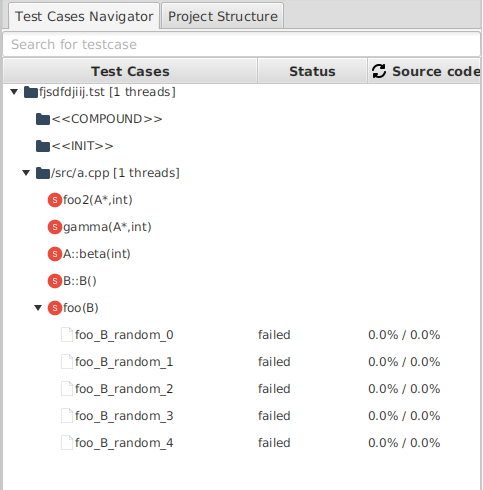
\includegraphics[width=\linewidth]{images/effect.png}
		\end{minipage}
	\end{tabular}
	\caption{Ví dụ sự ảnh hưởng của hàm thiếu định nghĩa khi kiểm thử đơn vị tự động.}
	\label{fig:affect}
\end{figure}

Hình \ref{fig:affect} mô tả ví dụ về sự ảnh hưởng của hàm thiếu định nghĩa khi kiểm thử bởi các công cụ kiểm thử tự động. Trong đó, khi kiểm thử đơn vị cho hàm \tcode{foo} trong đoạn mã bên trái với đầu vào là đối tượng \tcode{param} - đối tượng của lớp \tcode{B}, kết quả thực thi các ca kiểm thử đều là \textit{failed}. Điều này dẫn đến công cụ không thể đánh giá được độ phủ mã nguồn kiểm thử, gây khó khăn trong việc đảm bảo chất lượng từ sớm. Trong đơn vị kiểm thử, đối tượng \tcode{param} gọi phương thức \tcode{stub} - phương thức chưa được cài đặt thân hàm. Điều này biến phương thức trở thành hàm thiếu định nghĩa. Do đó, khi sử dụng các công cụ kiểm thử tự động để kiểm thử đơn vị này, các ca kiểm thử đều không thể liên kết được, dẫn đến lỗi \textit{failed} như Hình \ref{fig:affect}. Thực trạng trên đã diễn ra trong quá trình phát triển phần mềm thực tế và được các công ty phát triển phần mềm quan tâm bởi sự ảnh hưởng lớn của nó trong quá trình kiểm thử và đảm bảo chất lượng phần mềm.

Hạn chế thứ hai khi áp dụng kĩ thuật kiểm thử tượng trưng động đó là sự phụ thuộc vào các hàm, thành phần khác trong mã nguồn khiến quá trình thực hiện kiểm thử tốn nhiều thời gian song kết quả độ phủ chưa cao. Ở mức độ kiểm thử đơn vị, quá trình kiểm thử nên tập trung vào đơn vị chính mà không cần quan tâm đến các phụ thuộc. Năm 2022, Trần Nguyên Hương và các cộng sự đã giới thiệu phương pháp sinh giả lập mã nguồn (stub) tự động AS4UT \cite{TUNG2022106821} nhằm giải quyết vấn đề trên. Tuy nhiên, phương pháp vẫn còn nhiều hạn chế khi chưa giải quyết được lời gọi phương thức. C++ là ngôn ngữ hướng đối tượng nên lời gọi phương thức đóng vai trò cầu nối cung cấp hành vi của một đối tượng. Các lời gọi như vậy có thể thay đổi giá trị thuộc tính của đối tượng gọi. Sự thay đổi này có thể dẫn đến những điều kiện trong đơn vị kiểm thử không thể thỏa mãn được nếu chỉ đơn thuần áp dụng phương pháp AS4UT. Bài toán trở nên phức tạp hơn khi phương thức được gọi có thể là hàm thiếu định nghĩa. Do đó, cần thiết phải nghiên cứu và phát triển giải pháp kiểm thử đơn vị tự động hiệu quả cho mã nguồn C/C++ chứa hàm thiếu định nghĩa. 

Để xử lý các hạn chế trên, khóa luận đề xuất một phương pháp nhằm tự động phát hiện và xử lý các hàm thiếu định nghĩa, đồng thời tự động sinh stub cho các lời gọi hàm trong quá trình kiểm thử đơn vị. Ý tưởng chính của phương pháp là cải tiến phương pháp kiểm thử đơn vị tự động truyền thống với hai bổ sung chính gồm (i) quá trình xử lý hàm thiếu định nghĩa sau quá trình phân tích mã nguồn, và (ii) bổ sung phương pháp xử lý lời gọi phương thức trong quá trình xử lý lời gọi hàm khi sinh stub tự động. Trong đó, quá trình xử lý hàm thiếu định nghĩa sẽ xác định danh sách các nguyên mẫu hàm thiếu định nghĩa cần quan tâm rồi sinh thân hàm giả cho chúng. Quy trình xử lý nguyên mẫu hàm được tách thành hai quy trình con gồm xử lý nguyên mẫu hàm cơ bản và nguyên mẫu hàm ảo. Sau đó, phương pháp đồng thời áp dụng kỹ thuật kiểm thử tượng trưng động và phương pháp sinh stub tự động để sinh dữ liệu kiểm thử tự động cho các đơn vị được kiểm thử. Điều này cho phép phương pháp đề xuất rút ngắn được thời gian chuẩn bị môi trường kiểm thử và đồng thời đạt được độ phủ mã nguồn cao hơn khi kiểm thử các dự án chứa mã nguồn thiếu định nghĩa. Qua đó cho thấy khả năng ứng dụng thực tiễn của phương pháp đề xuất trong các dự án thực tế để giảm thiểu chi phí kiểm thử và nâng cao chất lượng chương trình.

Phần còn lại của khóa luận được trình bày như sau. Chương~\ref{chap2} trình bày một số kiến thức cơ sở liên quan đến chủ đề sinh dữ liệu kiểm thử tự động cho các dự án C/C++, sinh giả lập mã nguồn tự động và làm rõ khái niệm hàm thiếu định nghĩa. Tiếp theo, Chương~\ref{chap3} chia sẻ chi tiết về phương pháp kiểm thử đơn vị tự động cho mã nguồn C/C++ chứa hàm thiếu định nghĩa. Chương~\ref{chap4} mô tả công cụ thực nghiệm và một số kết quả thực nghiệm đánh giá tính hiệu quả của phương pháp đề xuất. Cuối cùng, Chương \nameref{chap5} chia sẻ một số đúc kết về phương pháp đề xuất và thảo luận hướng nghiên cứu tiếp theo.